\section{Introduzione}
Un programma eseguito su un'architettura dotata di una singola unità di elaborazione centrale (CPU) può essere eseguita esclusivamente in maniera sequenziale (un'istruzione alla volta) in figura \ref{fig:single-computation}.
% TODO: \usepackage{graphicx} required
\begin{figure}[th]
	\centering
	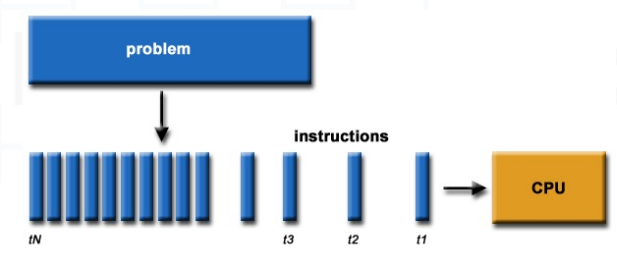
\includegraphics[width=0.7\linewidth]{img/single-computation}
	\caption{esecuzione su un'architettura dotata di una sola CPU.}
	\label{fig:single-computation}
\end{figure}
Nel senso più semplice, il \textbf{calcolo parallelo} è l'uso simultaneo di più risorse di calcolo per risolvere un problema computazionale. A differenza della soluzione sequenziale, l'esecuzione avviene su più di una CPU e il problema iniziale (il programma) viene suddiviso in sottoproblemi che a loro volta vengono suddivisi in una serie di istruzioni. L'esecuzione del programma avviene in maniera simultanea (figura \ref{fig:parallel-computation}).
\begin{figure}[th]
	\centering
	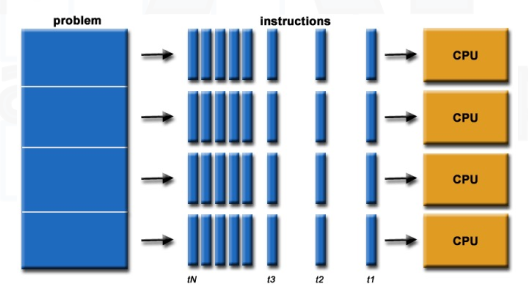
\includegraphics[width=0.7\linewidth]{img/parallel-computation}
	\caption{esecuzione parallela su un'architettura che supporta più di una CPU.}
	\label{fig:parallel-computation}
\end{figure}
